\documentclass[10pt,a4paper]{article}
\renewcommand{\baselinestretch}{1.0}
\usepackage{cite}
\usepackage[dvips]{graphicx}
\usepackage{psfrag}
\usepackage{color}
\usepackage[cmex10]{amsmath}
\usepackage{amsfonts}
\usepackage[font=footnotesize, captionskip=10pt]{subfig}
\usepackage{tikz}
\usepackage{flushend}
\usepackage{times}
\usepackage[margin=1.5cm]{geometry}
\usepackage[slovak]{babel}
\usepackage[utf8]{inputenc}
\usepackage[T1]{fontenc}
\usepackage[]{algorithm2e}


\pagestyle{empty}

\hyphenation{net-works}
\newtheorem{remark}{Remark}

\begin{document}

\title{Deep reinforcement learning using sparse distributed memory}
\author{Michal Chovanec, michal.nand@gmail.com \\
Peter Šarafín, peter.sarafin@gmail.com}
\date{}
\maketitle
\thispagestyle{empty}

%\noindent$^1$\ affiliation\\
%\noindent$^2$\ affiliation\\

\noindent {\bf Keywords:} reinforcement learning, function approximation, SARSA, Q-learning, sparse distributed memory, robotics, neural network

\noindent {\bf Abstract:}
In this paper we present advanced sparse distributed memory (ASDM) (based on original Kenerva's research \cite{bib:sdm_01}\cite{bib:sdm_02}\cite{bib:sdm_03}).
We designed deep unsupervised features extraction algorithm combined with linear combination of features
to store Q values of SARSA algorithm.
On three experiments we show ability of to use sparse coding for Q-value approximation.
Those experiments include ASDM topology experiments (including convolutional ASDM), noise imunity
and learning speed in virtaul environment. {\bf TODO} and finally - line following robot experiment.

\section{Introduction}

Reinforcement learning is well known method {\bf TODO citovat Watkinsa} to solve Markovov decission problems {\bf TODO citovat co to je}.
Commonly used algorithms are Q-learning and SARSA (equation \ref{eq:rl_sarsa_learning}).
This function is handling information about suitablity action $a(n)$ in state $s(n)$.

\begin{equation}
  \label{eq:rl_sarsa_learning}
  Q'(s, a) = (1-\alpha)Q(s, a) + \alpha \Big(R(s, a) + \gamma Q(s', a') \Big)
\end{equation}

For small state spaces (usually only in examples) a table can be used to store $Q$ values.
For large state spaces - with hundreds of state features, the approximation is necessary.
Well known are linear combinations of basis functions {\bf TODO citovat} or feed forward neural networks {\bf citovat}.

Reccurent character of equation \ref{eq:rl_sarsa_learning} makes learning process inefficient,
and slow.

Our idea is focused on linear combination of learned features. Deep features extraction
part is learned unsupervised. On last stage is processed linear combination of features, and
this part is learned supervised. Because of linear character, this part is learning fast.
Another benefit from features extraction leads to build learning system with ability to use
past knowledges to make new conclusion in situation which was never observed before, but have similar features like some past situation.

Those features should be sparse, reasons for sparsness
are explained in well cited paper such \cite{bib:sparse_01}, \cite{bib:sparse_02},
and in medical papers focused on research of primary and visual cortex \cite{bib:sparse_03}, \cite{bib:sparse_04},
\cite{bib:sparse_05}, \cite{bib:sparse_06}. Sparse coding uses linear combination of
few selected words from dictionary to represents input, this shows image \ref{img:Sparse representation principle}.

\begin{figure}[!h]
  \centering
  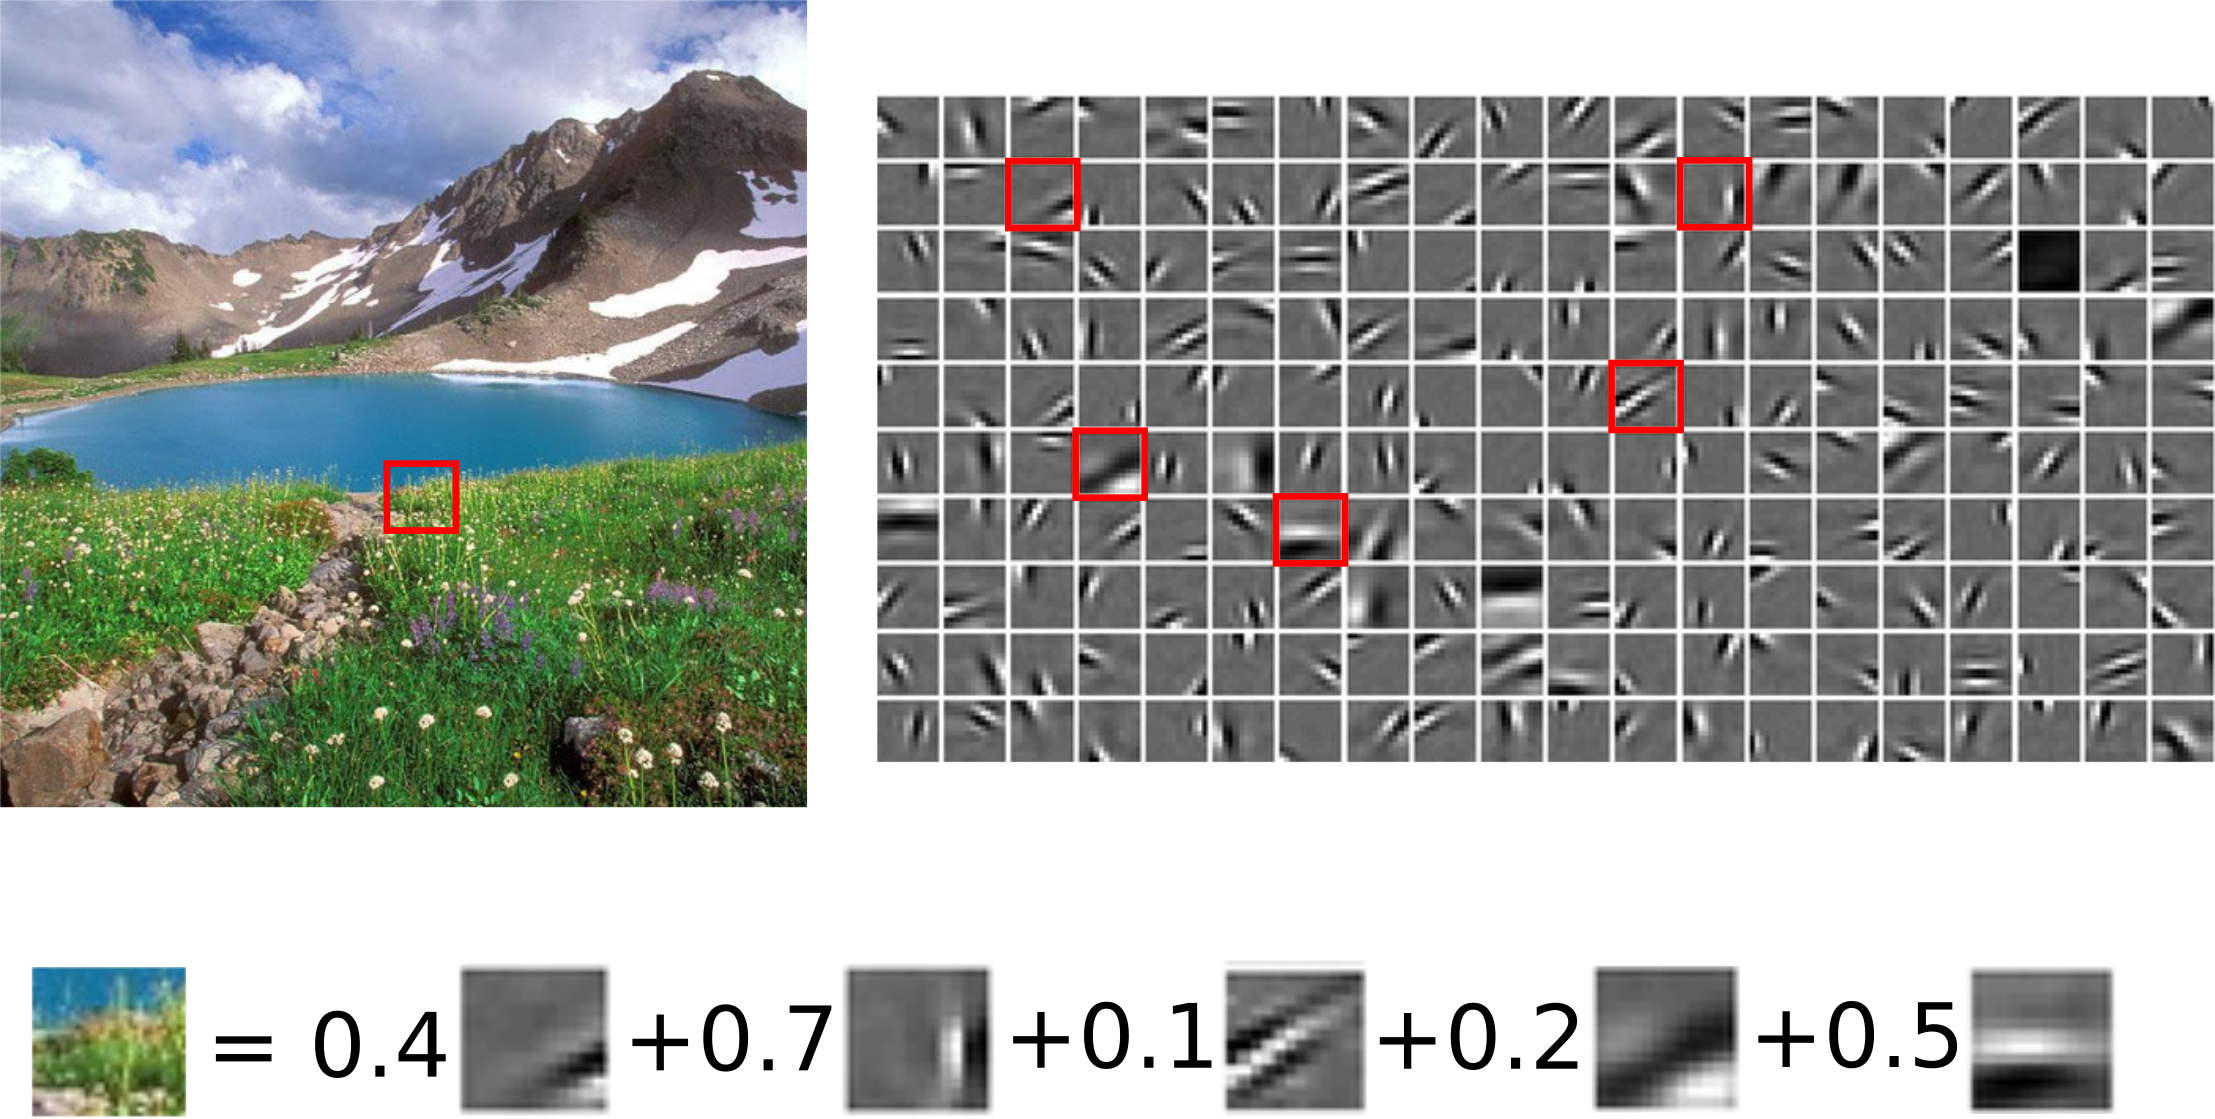
\includegraphics[scale=0.3]{../diagrams/sparse_dictionary.png}
  \caption{Sparse representation principle}
  \label{img:Sparse representation principle}
\end{figure}


\section{ASDM algorithm}

Based on K-SVD algorithm {\bf TODO citovat}.
Optimization problem formalisation :
\begin{align*}
E(w, y) &= \sum_{k=0}^{K-1} \left\Vert x_k - wy_k \right\Vert^2_2 + \lambda_0 \left\Vert y_k \right\Vert^2_1 + \lambda_1 \left\Vert w \right\Vert^2_{2,1} \\
&\text{subject to} \quad y_{ki} > 0
\end{align*}

\begin{itemize}
  \item
      reconstruction condition
      \color{red}
      \begin{align*}
      \left\Vert x_k - wy_k \right\Vert^2_2
      \end{align*}
      \color{black}


  \item
      $y_k$ sparsity condition
      \color{green}
      \begin{align*}
      \lambda_0 \left\Vert y_k \right\Vert^2_1
      \end{align*}
      \color{black}


  \item
      $w$ sparsity condition
      \color{blue}
      \begin{align*}
      \lambda_1 \left\Vert w \right\Vert^2_{2,1}
      \end{align*}
      \color{black}
\end{itemize}


Our goal is to approximate function $y = f(x)$, where $x,y \in \!R$ are vectors.
The $x$ is input with size $N$, and have usually huge dimension (f.e. ten's of sensors, hundreds of camera pixels ...).
Output $y$ with size $M$ can be class in classification problem, or any required value to approximate, usually with
significantly lower dimension than $x$.

Learning process is done in two steps : \\
{\bf unsupervised learning}, where Oja's rule is used to estimate input weights \\
{\bf supervised learning}, where gradient descent is used to estimate output weights \\

\begin{algorithm}
 \KwData{W, depth, X}
 \KwResult{sparse representation Y, features matrix weights W }
 initialization  \\
                $W \gets random$, $R \gets X$ \\
                $\eta$ learning rate, $\epsilon$ shrink value \\
 \For{j from 0 to depth}
 {
  \color{blue}
  $best = \arg\max\limits_{i} W[i] R $ \\
  \color{red}
  $d = ReLU (\frac{W[best] R}{\Vert W[best]\Vert^2_2})$ \\
  $Y[best] = d$ \\
  \color{black}
  \For{i from 0 to size(R)}
  {
    $dw = d(R[i] - W[best][i])$ \\
    $W[best][i] = W[best][i] + \eta dw$ \\

    $W[best][i] = shrink(W[best][i], \epsilon)$

    \color{green}
    R[i] = R[i] - d*W[best][i]
  }
 }
\end{algorithm}




\begin{figure}[!htb]
  \centering
  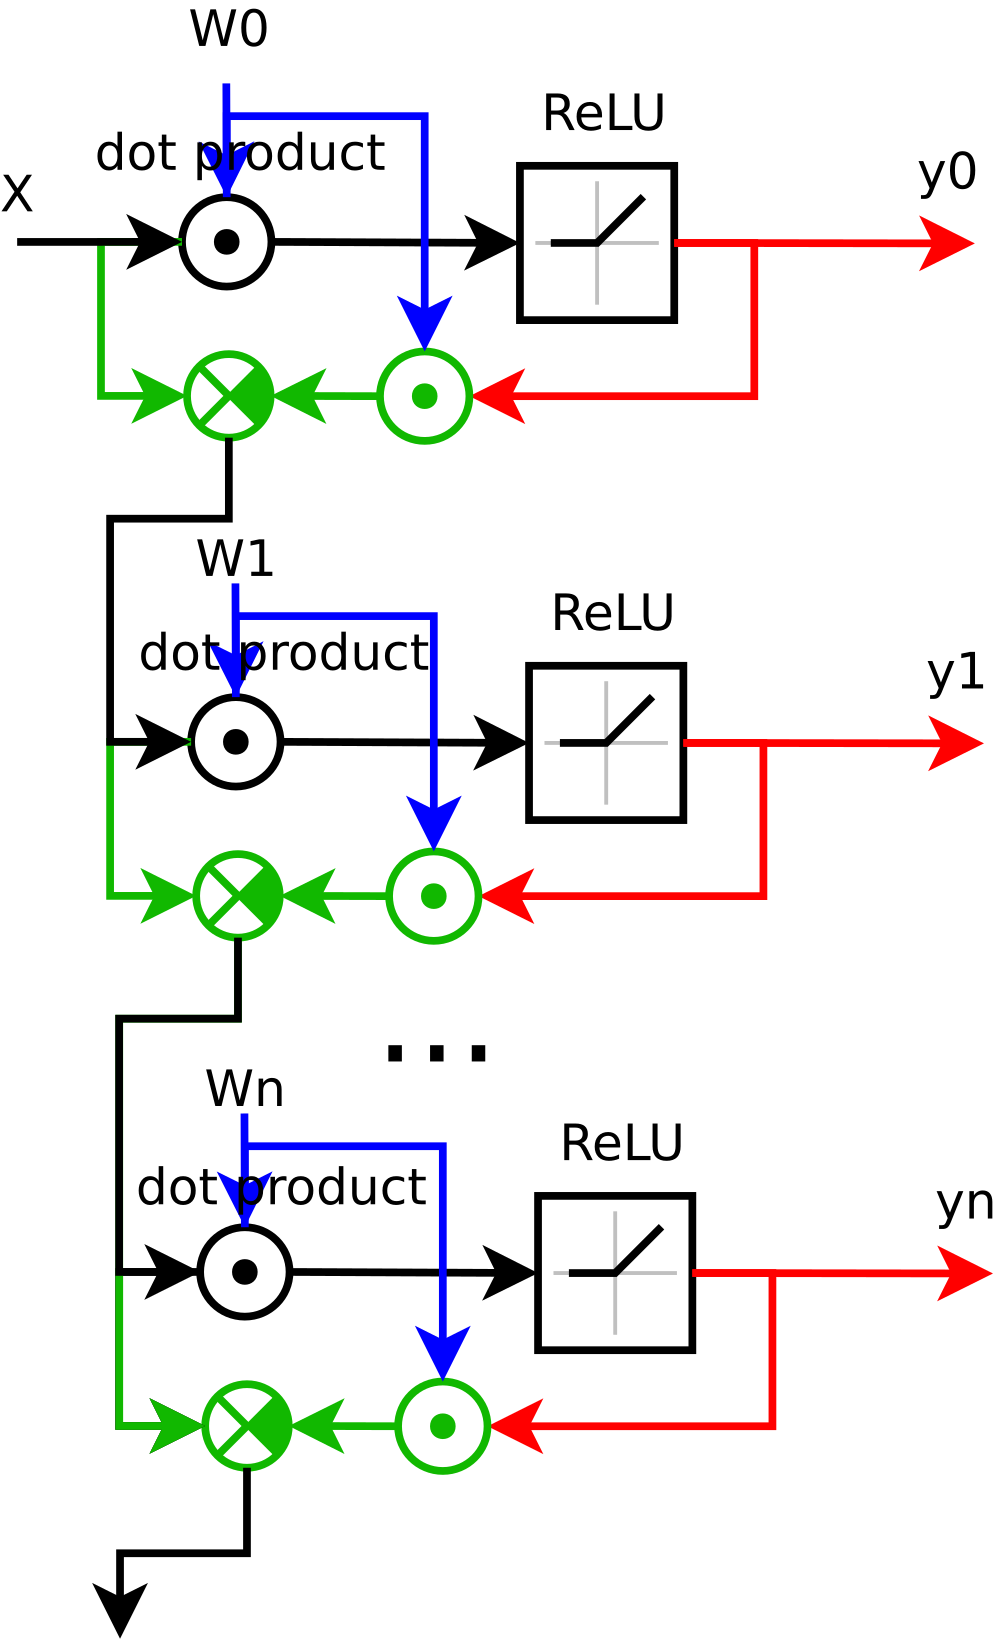
\includegraphics[scale=0.13]{../diagrams/features_layer_01.png}
  \caption{Algorithm working princple}
  \label{img:Algorithm working princple}
\end{figure}


\begin{figure}[!htb]
  \centering
  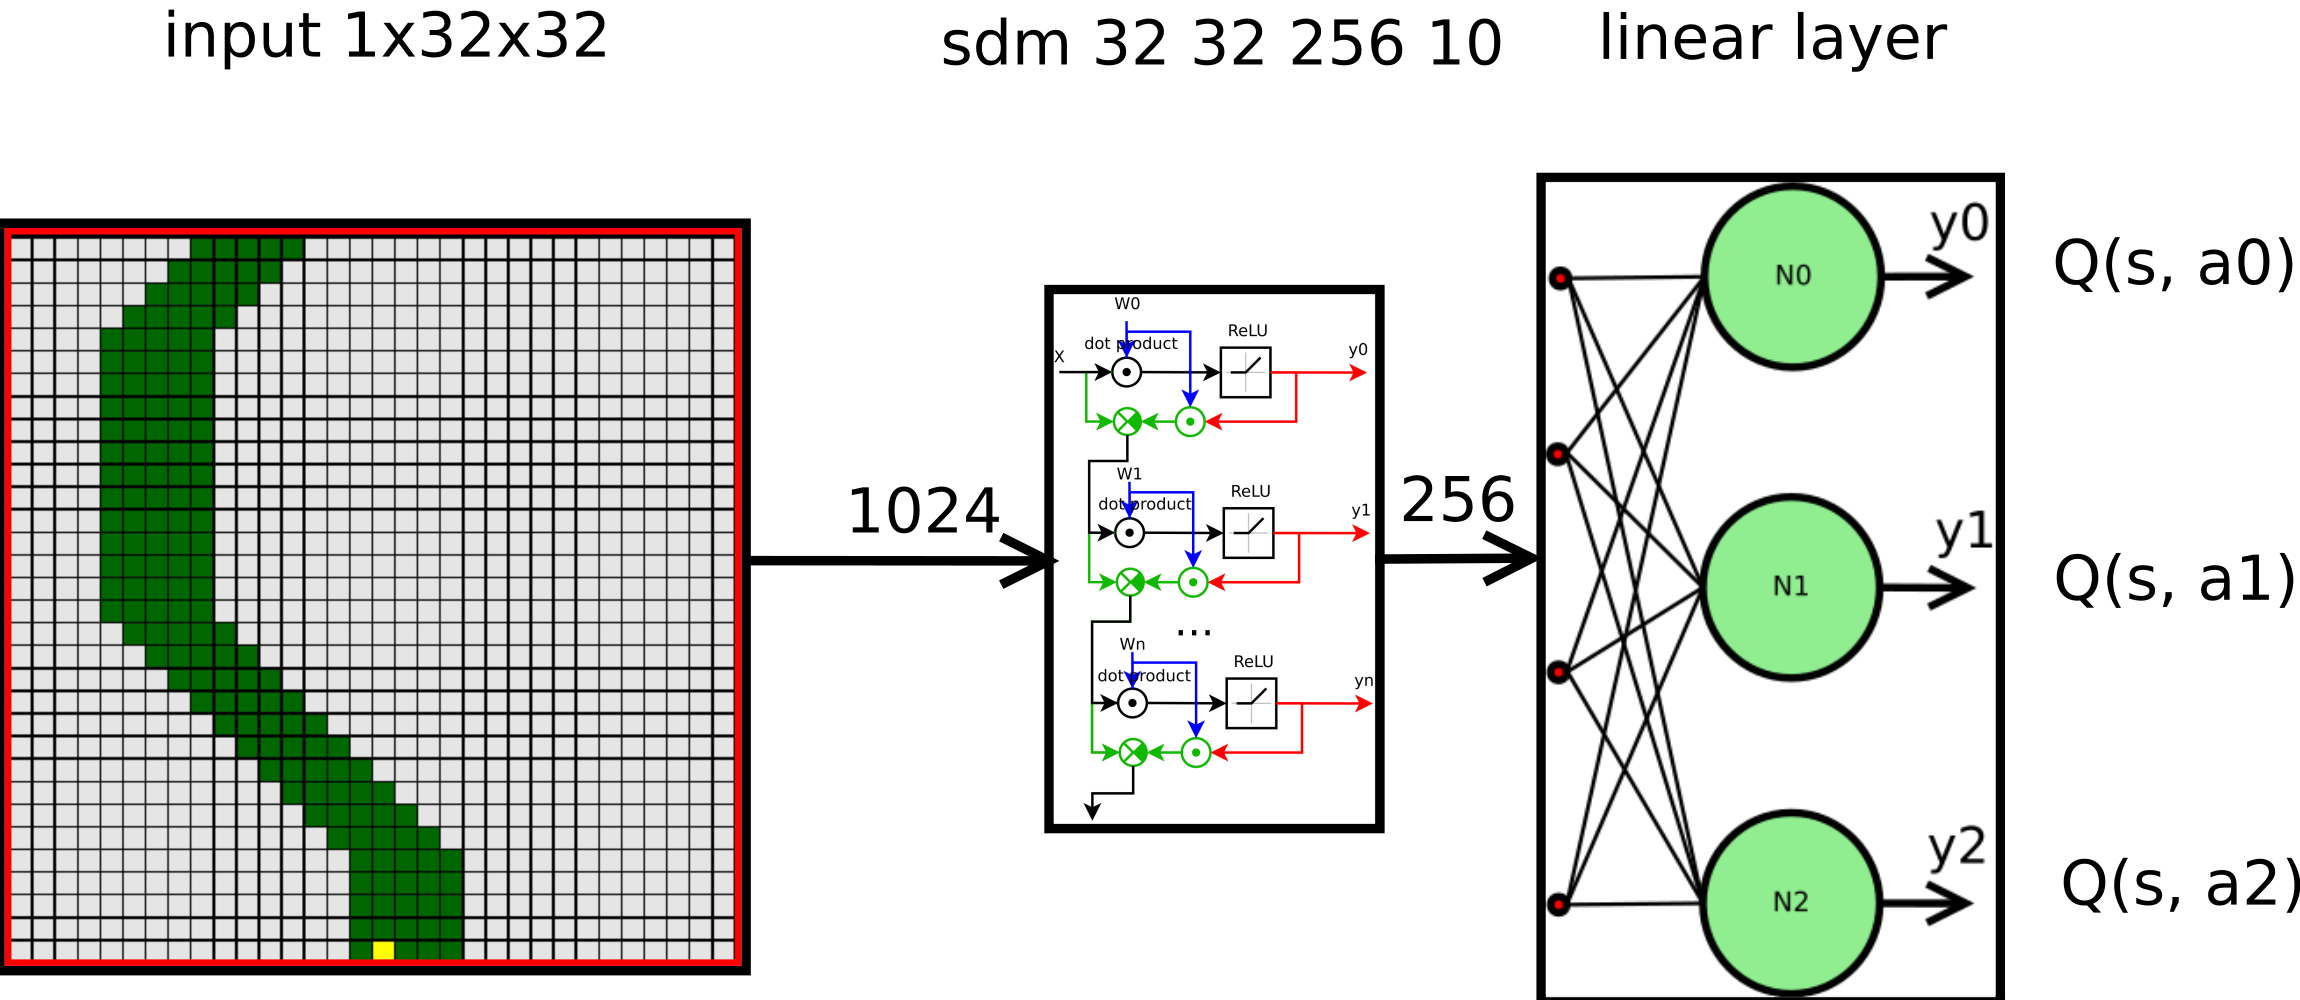
\includegraphics[scale=0.18]{../diagrams/convolution_01.png}
  \caption{Basic ASDM topology}
  \label{img:Basic ASDM topology}
\end{figure}


\begin{figure}[!htb]
  \centering
  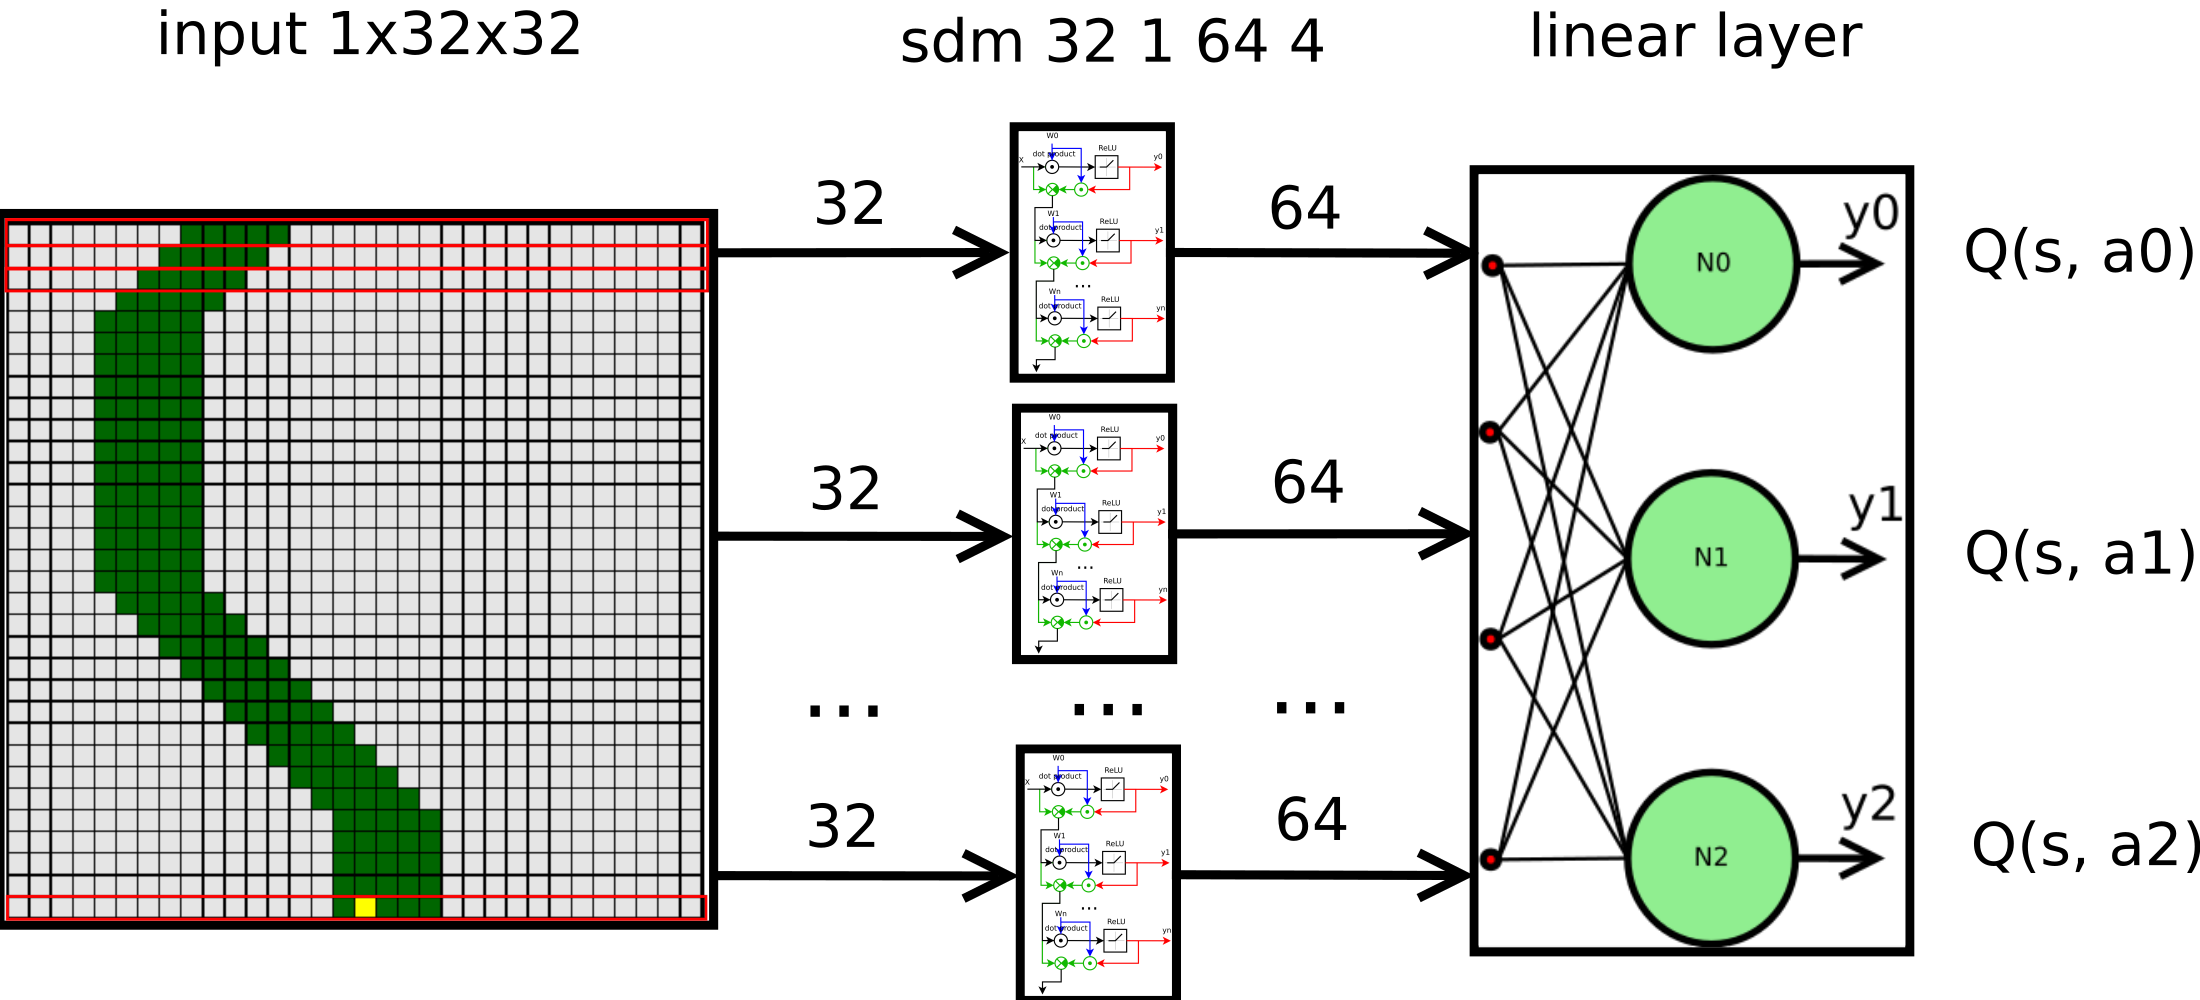
\includegraphics[scale=0.18]{../diagrams/convolution_02.png}
  \caption{ASDM + Convolution topology}
  \label{img:ASDM + Convolution topology}
\end{figure}

\begin{figure}[!htb]
  \centering
  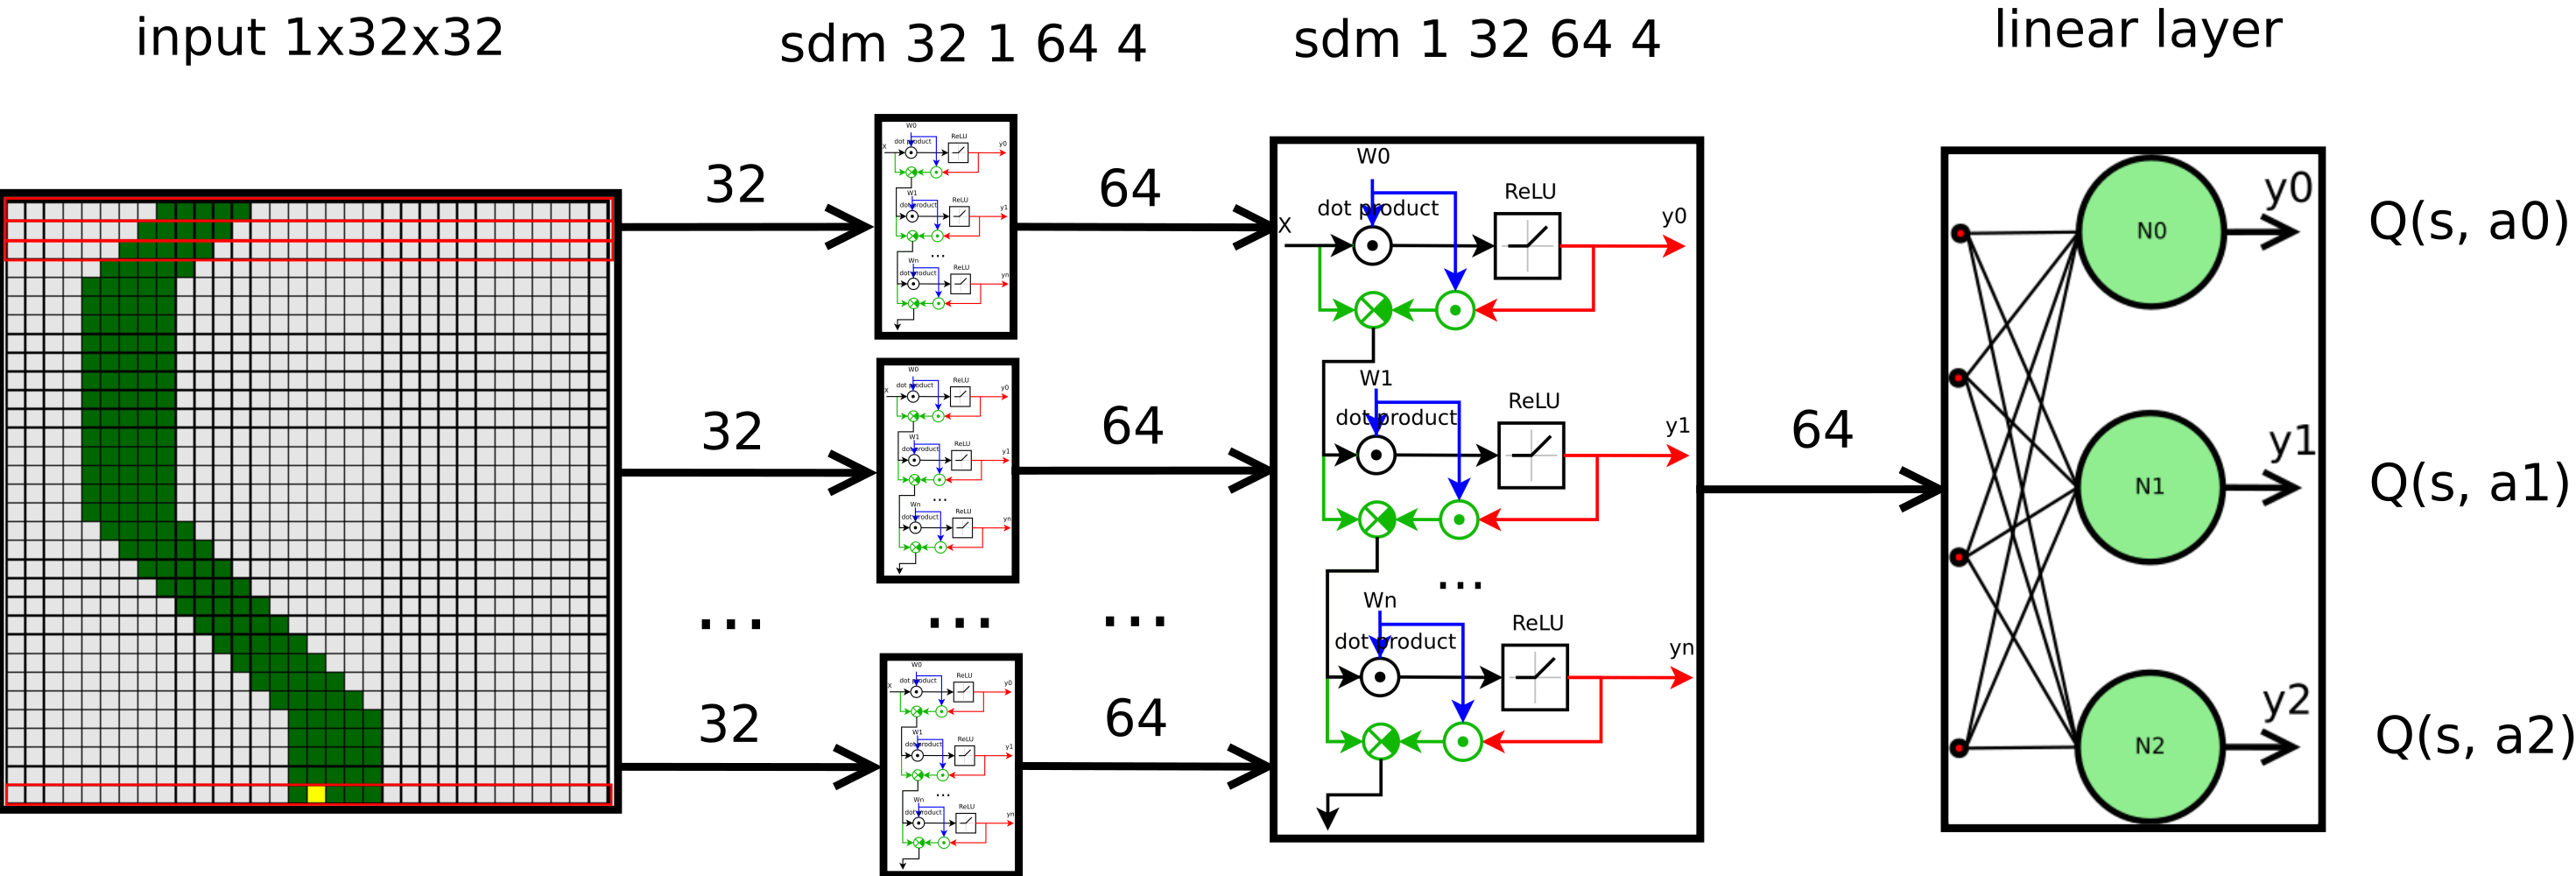
\includegraphics[scale=0.18]{../diagrams/convolution_03.png}
  \caption{ASDM + Convolution topology + Deep layer}
  \label{img:ASDM + Convolution topology + Deep layer}
\end{figure}




\newpage
\section{Experimental results}

\section{Mouse and food}

\begin{itemize}
  \item state : vector $64x\{0, 1\}$, 1 if mouse on field
  \item action : left, right, up, down
  \item reward : +1 for target hit, -1 for red hit
\end{itemize}

\begin{figure}[!htb]
  \centering
  \includegraphics[scale=0.27]{../pictures/mouse_desc.png}
  \caption{Mouse experiment description}
  \label{img:Mouse experiment description}
\end{figure}

\begin{figure}[!htb]
\centering
\begin{minipage}{.5\textwidth}
  \centering
  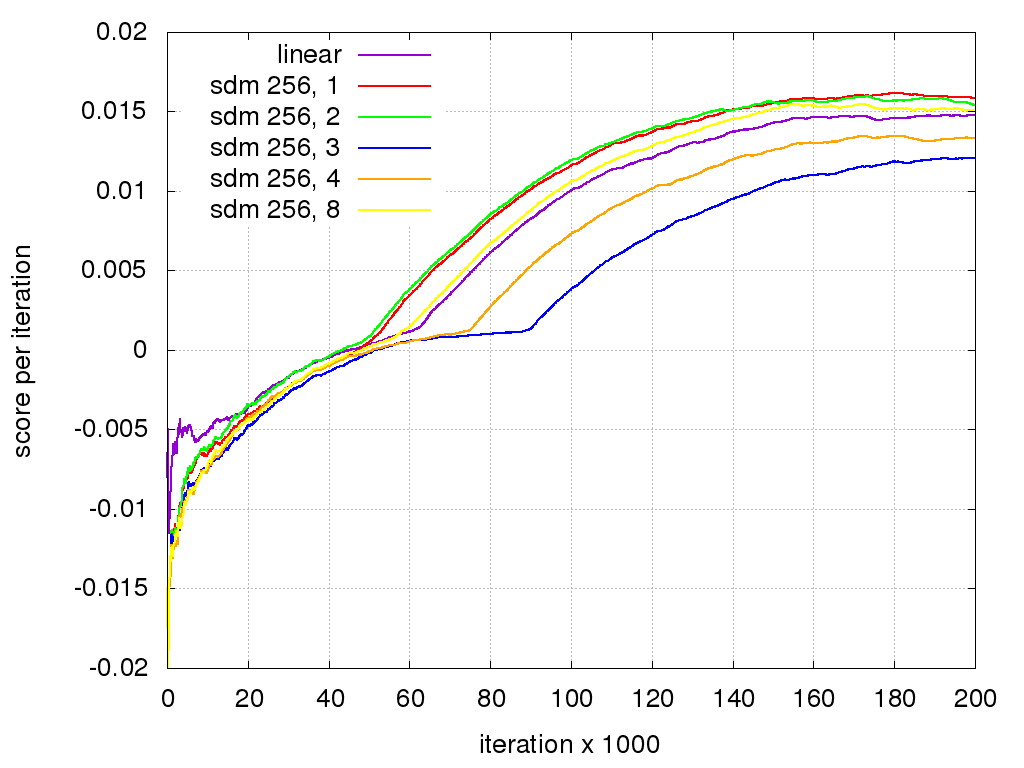
\includegraphics[width=1.0\linewidth]{{../results/mouse_result/progress_per_iteration_0.000}.png}
  \captionof{figure}{Score progress rate, for state noise 0.0}
\end{minipage}%
\begin{minipage}{.5\textwidth}
  \centering
  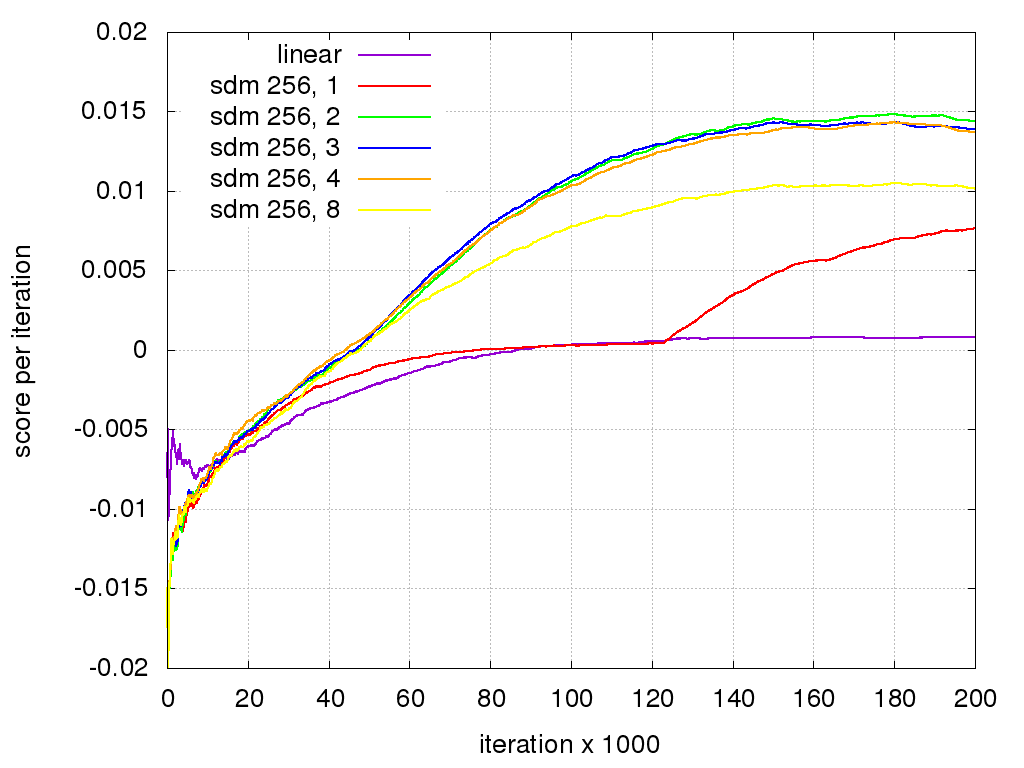
\includegraphics[width=1.0\linewidth]{{../results/mouse_result/progress_per_iteration_0.100}.png}
  \captionof{figure}{Score progress rate, for state noise 0.1}
\end{minipage}
\end{figure}

\begin{figure}[!htb]
{\bf visited fields rate for linear approximator}
\centering
\begin{minipage}{.5\textwidth}
  \centering
  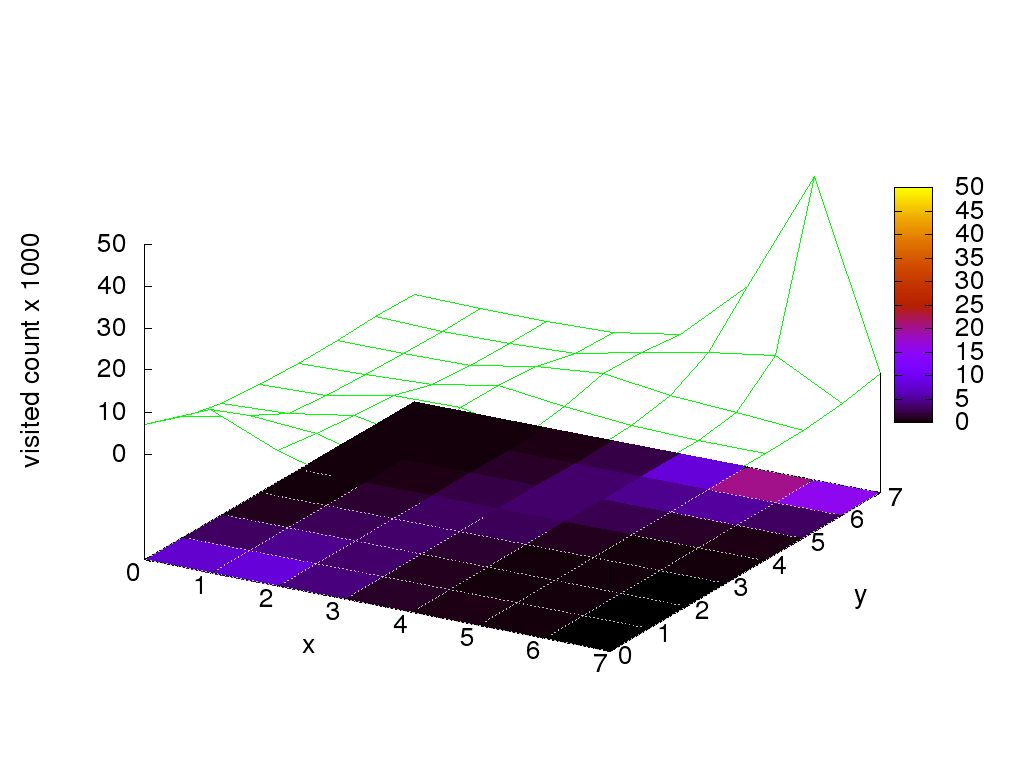
\includegraphics[width=1.0\linewidth]{{../results/mouse_result/linear_0.000__visited_fields}.png}
  \captionof{figure}{Visited field rate, state noise 0.0}
\end{minipage}%
\begin{minipage}{.5\textwidth}
  \centering
  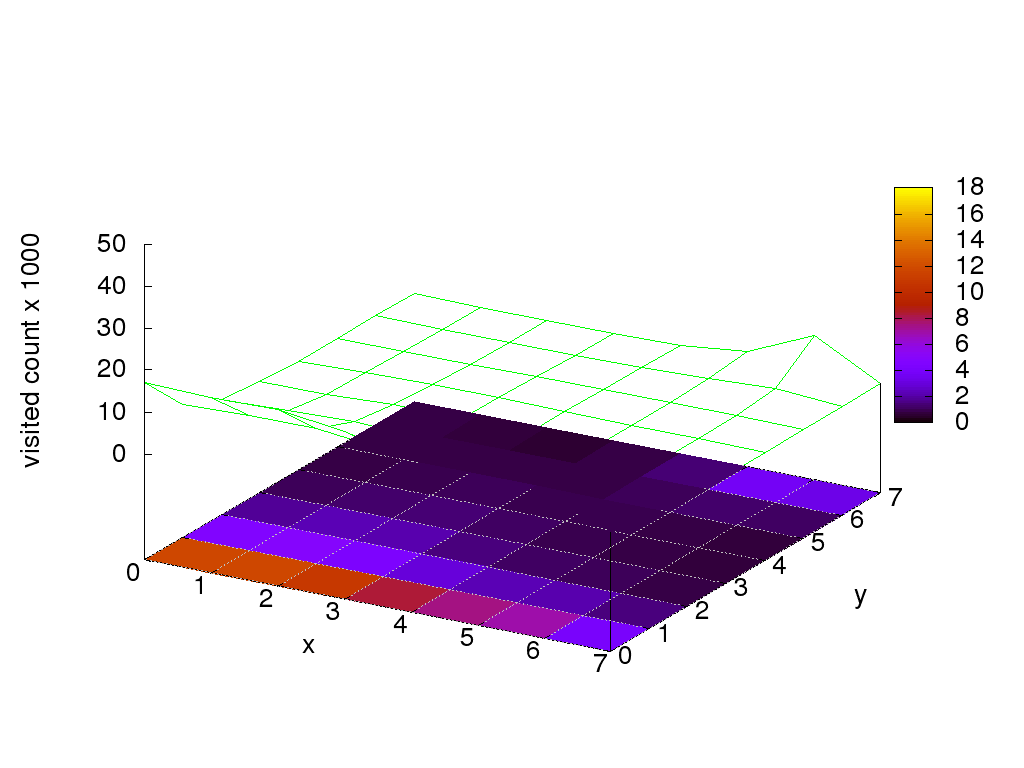
\includegraphics[width=1.0\linewidth]{{../results/mouse_result/linear_0.100__visited_fields}.png}
  \captionof{figure}{Visited field rate, state noise 0.1}
\end{minipage}
\end{figure}

\begin{figure}[!htb]
{\bf visited fields rate for SDM approximator}
\centering
\begin{minipage}{.5\textwidth}
  \centering
  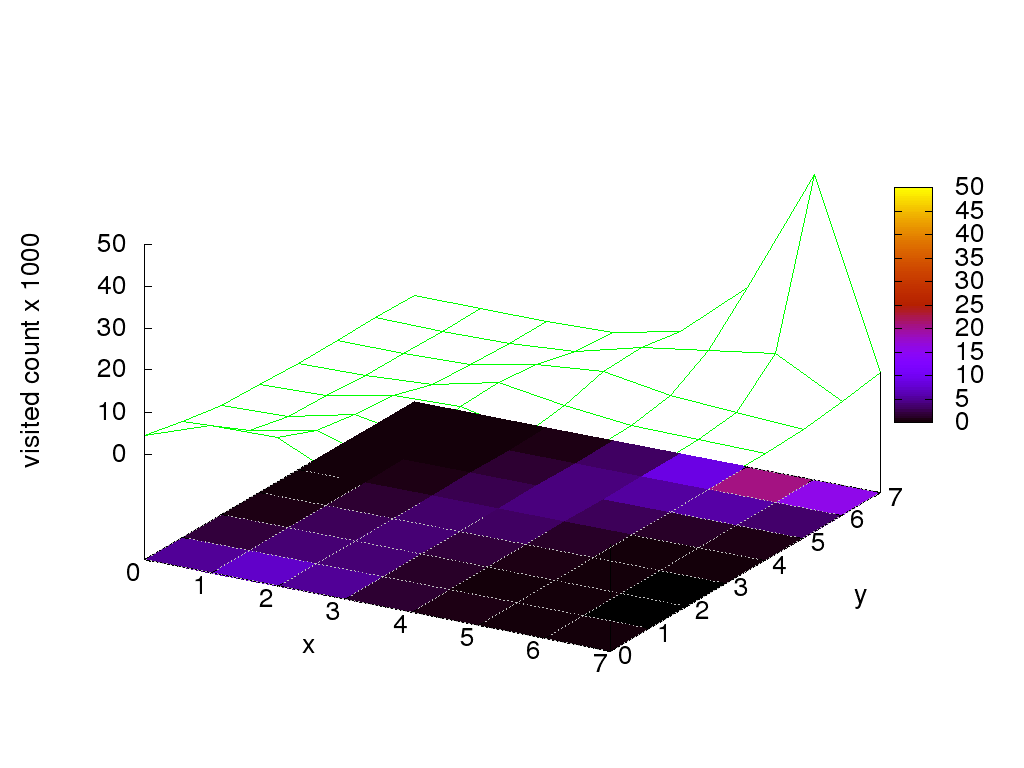
\includegraphics[width=1.0\linewidth]{{../results/mouse_result/sdm_0.000_256_2_visited_fields}.png}
  \captionof{figure}{Visited field rate, state noise 0.0}
\end{minipage}%
\begin{minipage}{.5\textwidth}
  \centering
  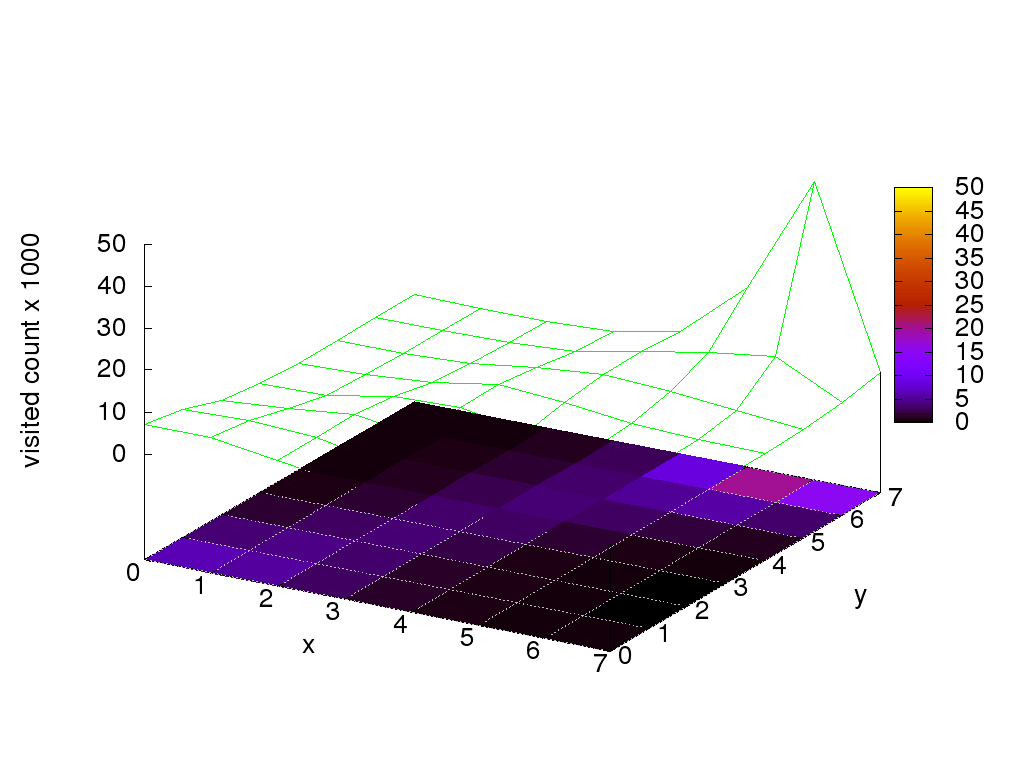
\includegraphics[width=1.0\linewidth]{{../results/mouse_result/sdm_0.100_256_2_visited_fields}.png}
  \captionof{figure}{Visited field rate, state noise 0.1}
\end{minipage}
\end{figure}


\section{Virtual line follower}


\begin{figure}[!htb]
  \centering
  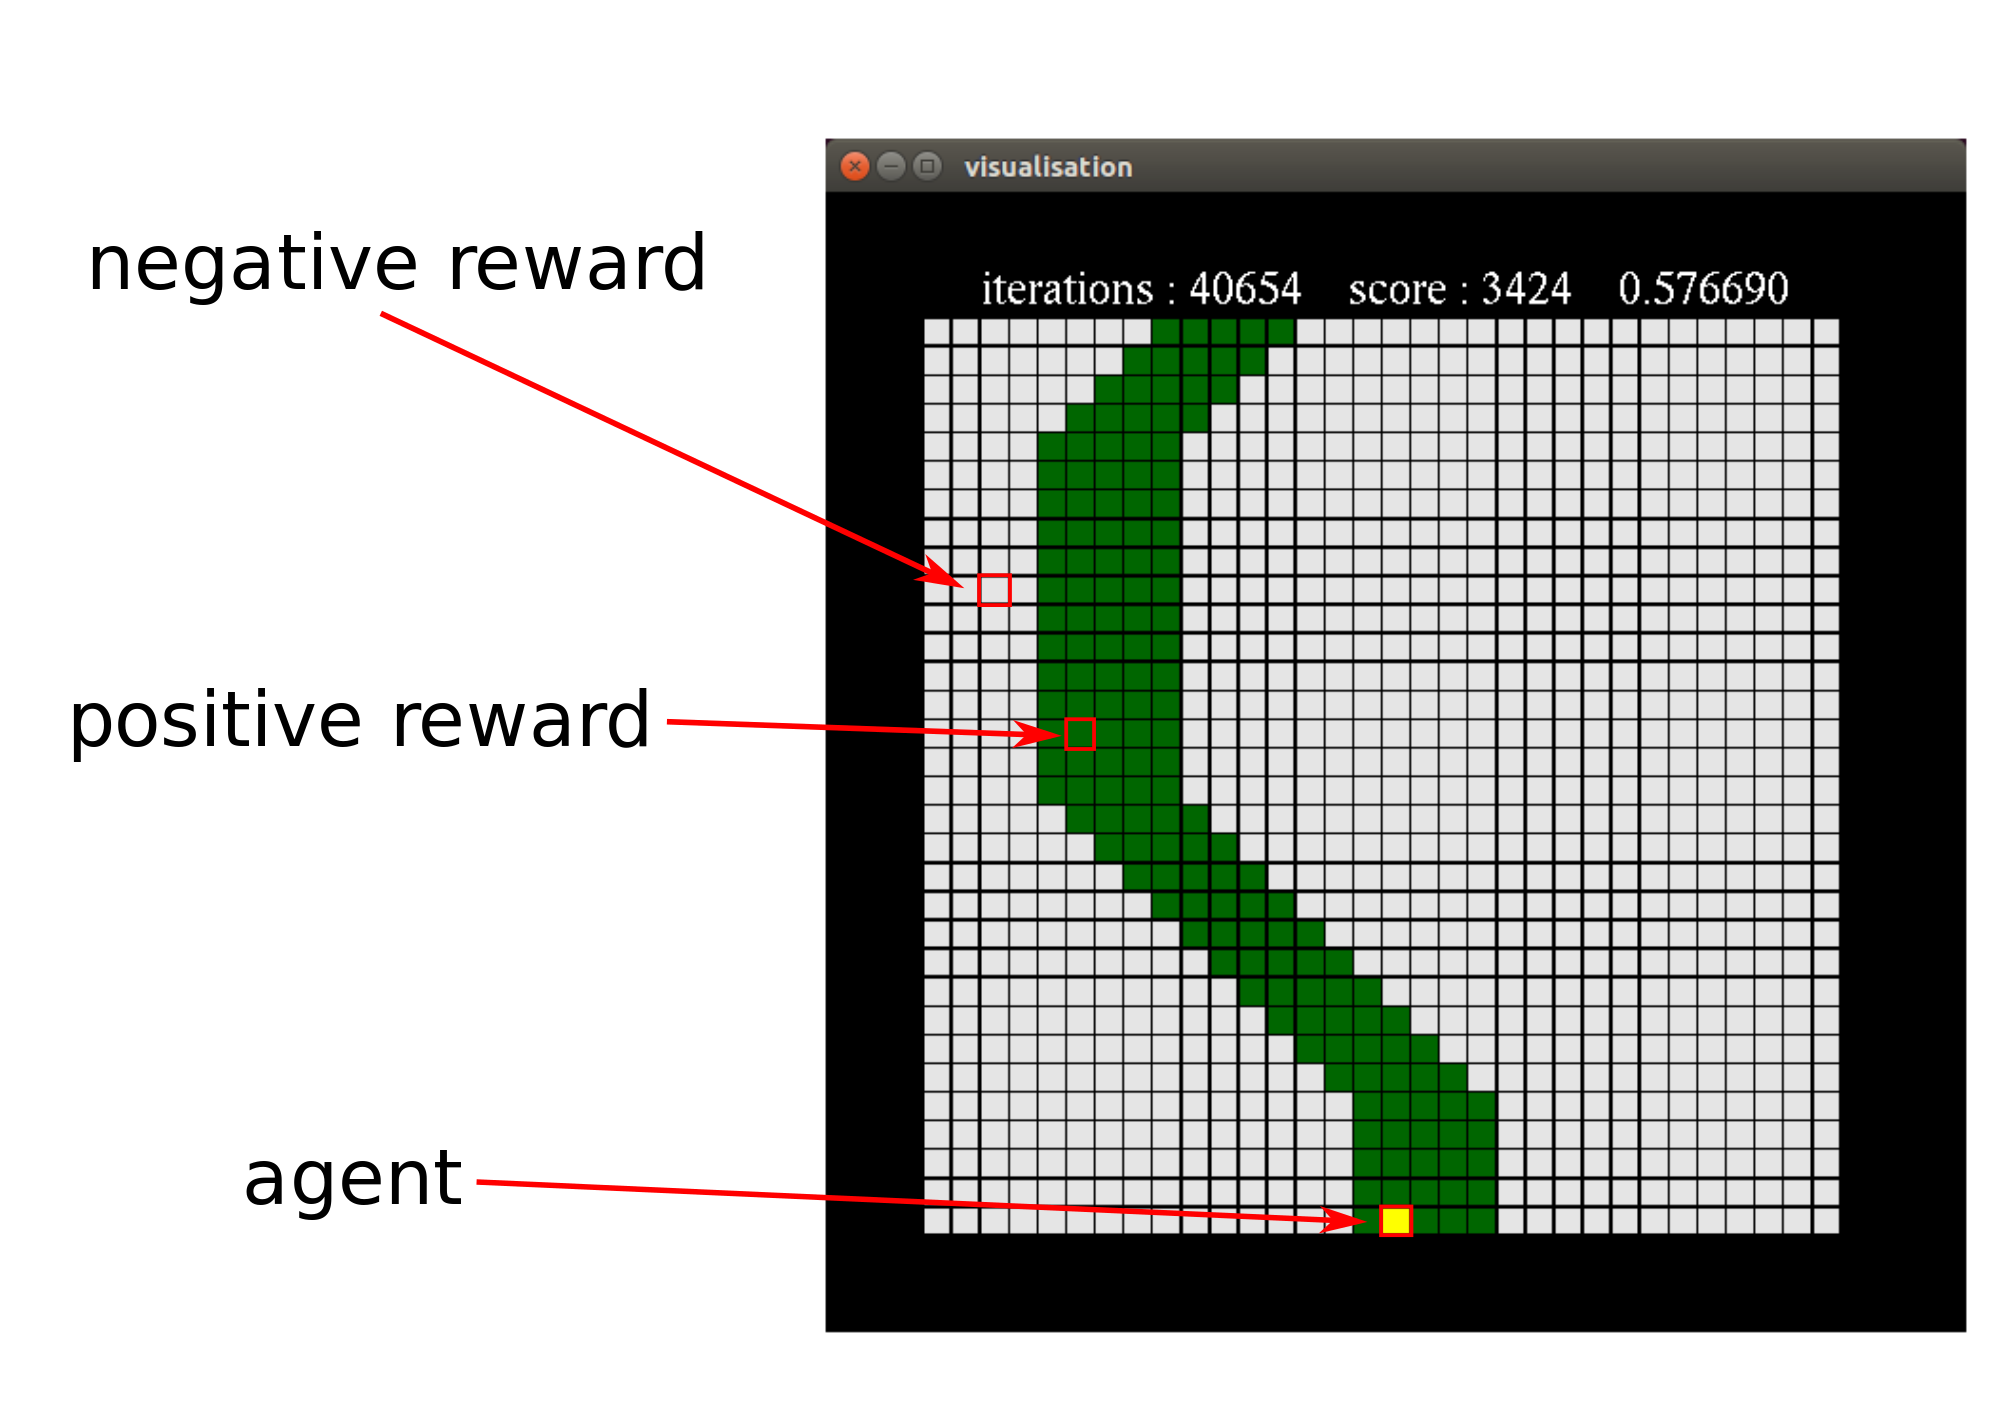
\includegraphics[scale=0.15]{../pictures/rl_race_desc.png}
  \caption{Virtual line follower description}
  \label{img:Virtual line follower description}
\end{figure}


\begin{itemize}
\item motion equations of robot
  \begin{align*}
  a(n) &= \{-1, 0, 1\} \\
  v(n) &= \alpha r(n-1) + (1.0 - \alpha) a(n) \\
  p(n) &= p(n-1) + v(n)
  \end{align*}

\item reward
\[
    r(n)=
\begin{cases}
    +1,& \text{if green field}\\
    -1, & \text{otherwise}
\end{cases}
\]
\end{itemize}


\begin{figure}[!htb]
{\bf summary results for virtual line follower}
\centering
\begin{minipage}{.5\textwidth}
  \centering
  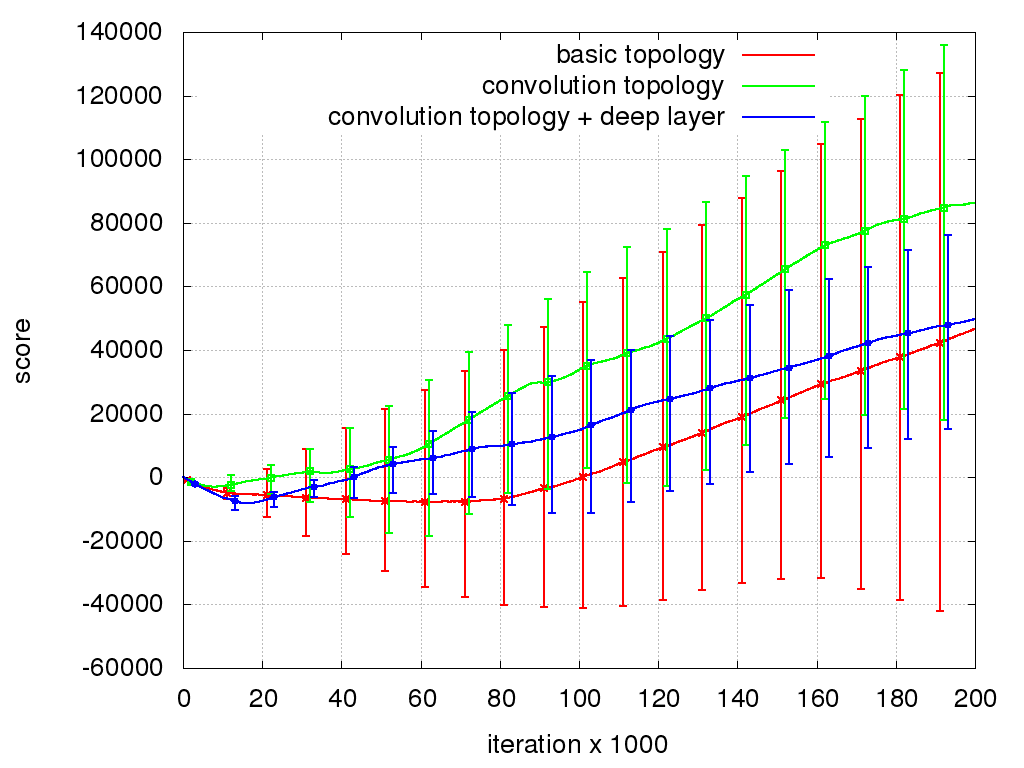
\includegraphics[width=1.0\linewidth]{../results/rl_race_experiment/deep_progress.png}
  \captionof{figure}{Total score}
\end{minipage}%
\begin{minipage}{.5\textwidth}
  \centering
  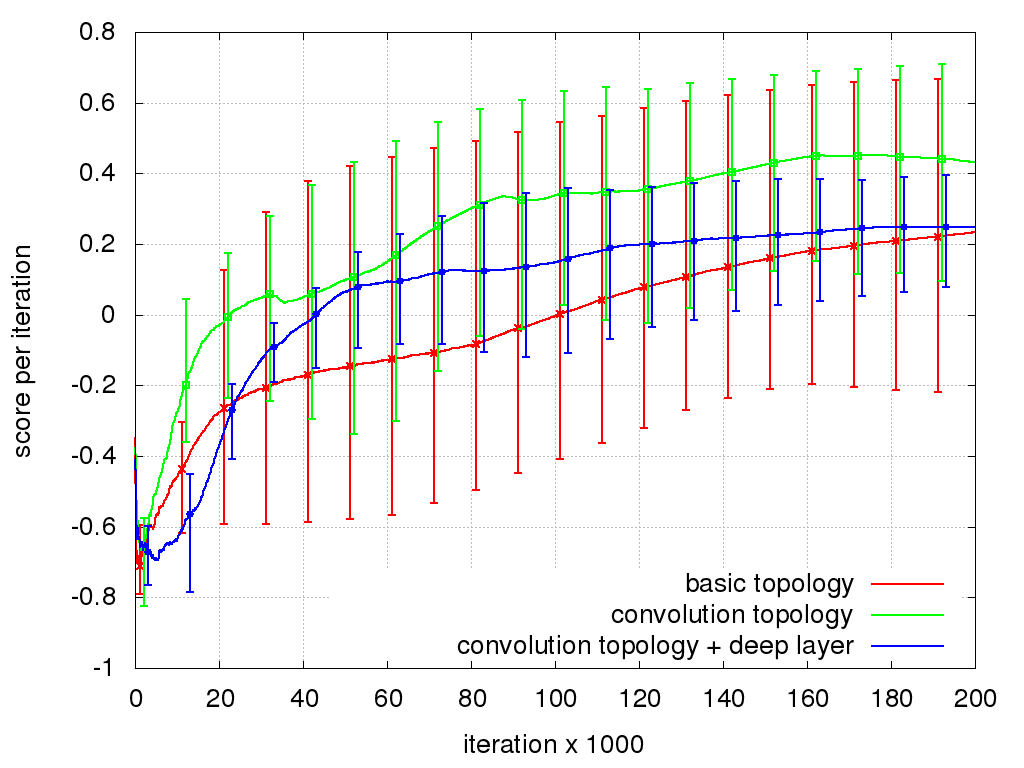
\includegraphics[width=1.0\linewidth]{../results/rl_race_experiment/deep_progress_per_iteration.png}
  \captionof{figure}{Progress per iteration}
\end{minipage}
\end{figure}


\section{Worms}


\begin{figure}[!htb]
  \centering
  \includegraphics[scale=0.27]{../pictures/sdm_demo_desc.png}
  \caption{Multiple worms testing application}
  \label{img:Multiple worms testing application}
\end{figure}



\begin{figure}[!htb]
\centering
\begin{minipage}{.5\textwidth}
  \centering
  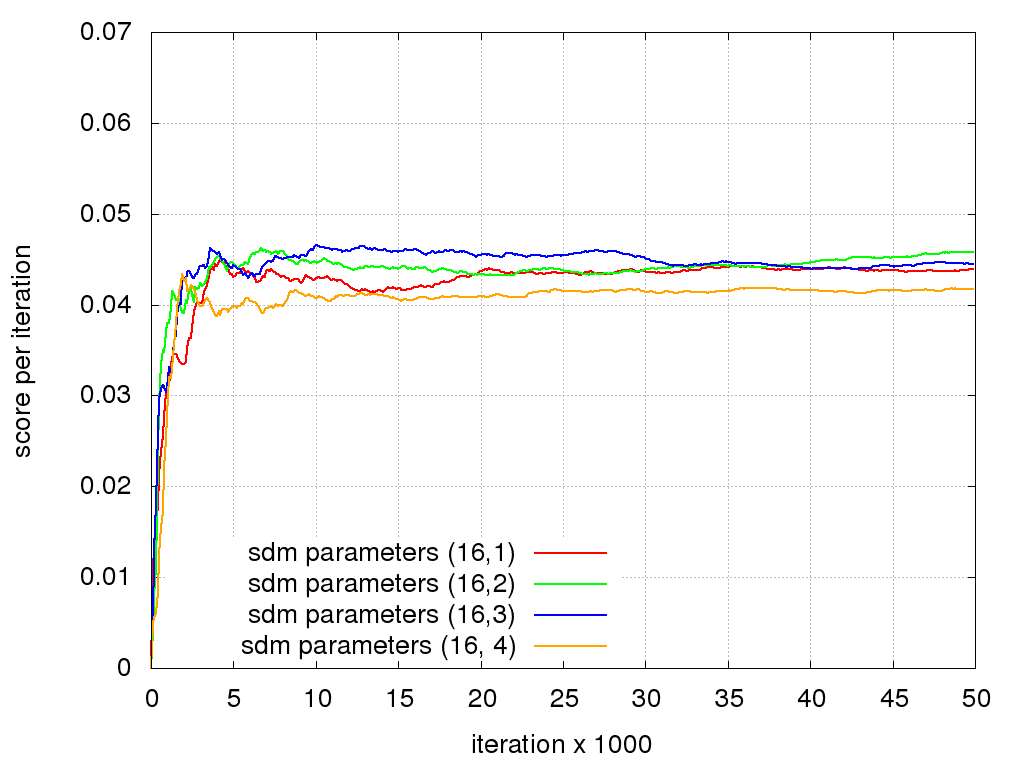
\includegraphics[width=1.0\linewidth]{{../results/worms_result/progress_experiment_/progress_per_iteration_16}.png}
\end{minipage}%
\begin{minipage}{.5\textwidth}
  \centering
  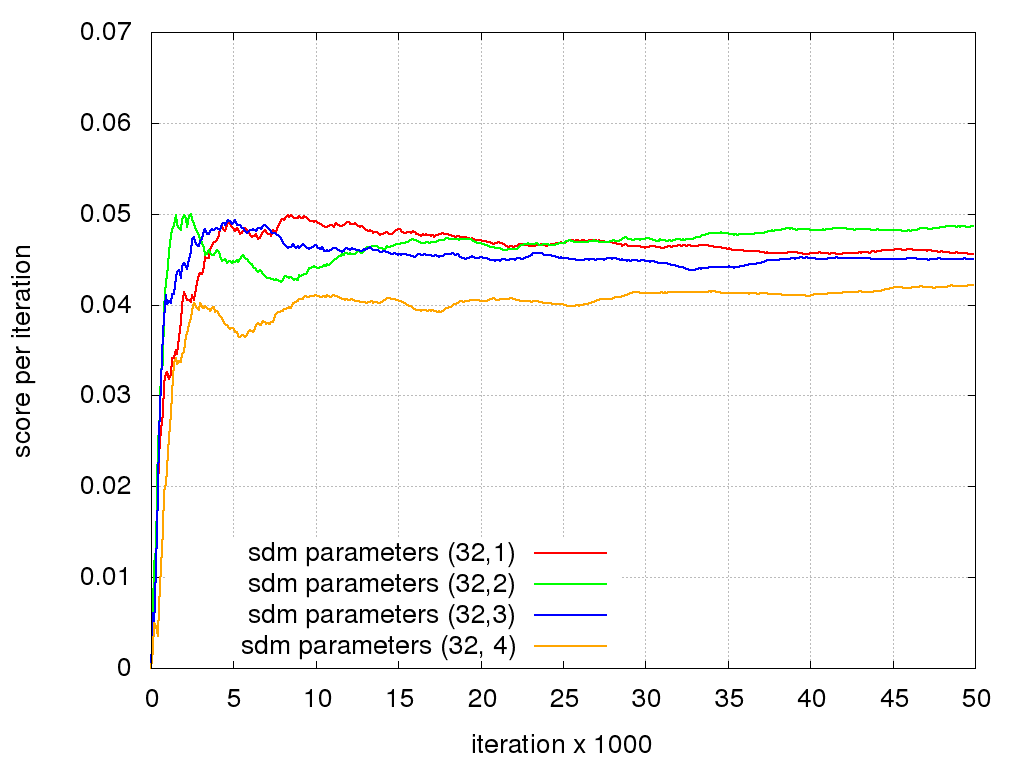
\includegraphics[width=1.0\linewidth]{{../results/worms_result/progress_experiment_/progress_per_iteration_32}.png}
\end{minipage}
\caption{Memory size and activity results}
\end{figure}



\begin{figure}[!htb]
\centering
\begin{minipage}{.5\textwidth}
  \centering
  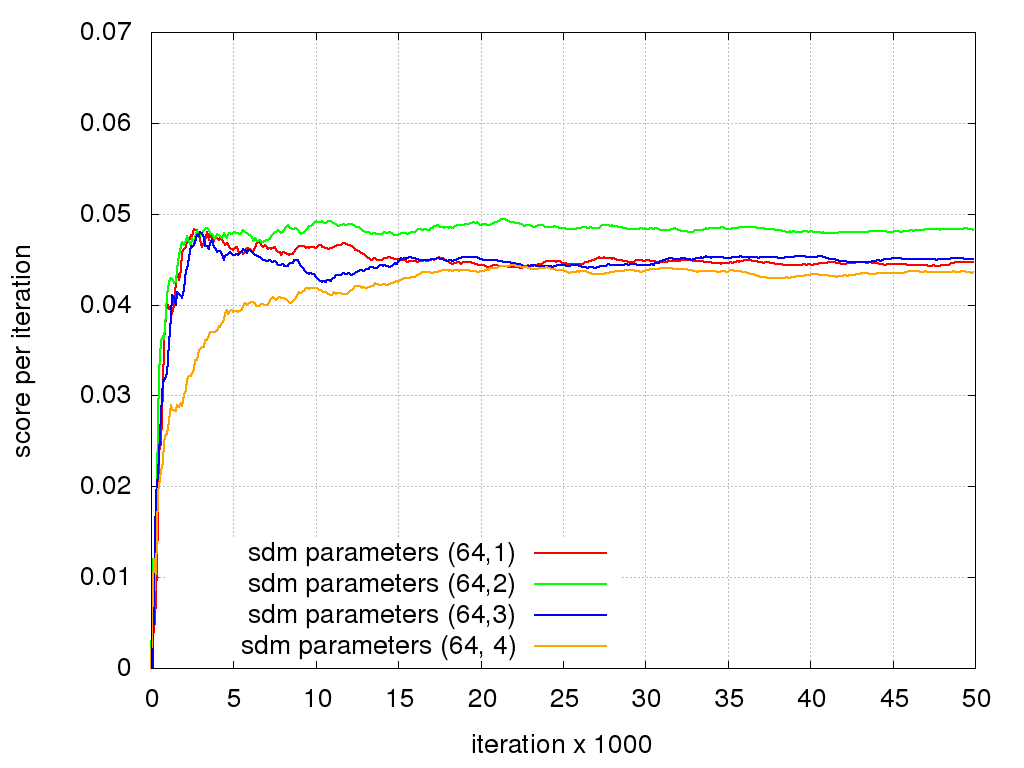
\includegraphics[width=1.0\linewidth]{{../results/worms_result/progress_experiment_/progress_per_iteration_64}.png}
\end{minipage}%
\begin{minipage}{.5\textwidth}
  \centering
  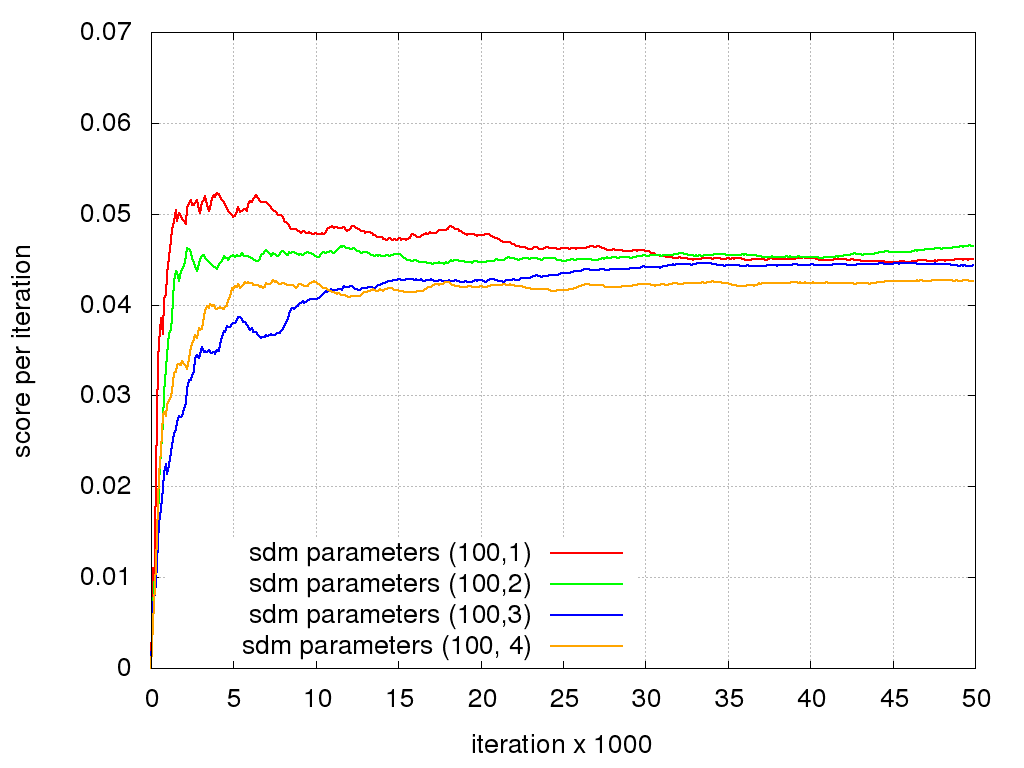
\includegraphics[width=1.0\linewidth]{{../results/worms_result/progress_experiment_/progress_per_iteration_100}.png}
\end{minipage}
\caption{Memory size and activity results}
\end{figure}



\newpage
\subsection{Conclusion}

\newpage
\bibliographystyle{IEEEtran}
\bibliography{bib}

\begin{thebibliography}{4}

\bibitem{bib:sdm_01} M.J.Flynn, P.Kanerva, and N.Bhadkamkar, 1989, Sparse Distributed Memory: Principles and Operation
http://i.stanford.edu/pub/cstr/reports/csl/tr/89/400/CSL-TR-89-400.pdf

\bibitem{bib:sdm_02} David Rogers, 1988, NASA, KANERVA’S SPARSE DISTRIBUTED MEMORY: AN ASSOCIATIVE MEMORY ALGORITHM WELL SUITED TO THE CONNECTION MACHINE
https://pdfs.semanticscholar.org/9288/bb551f000348f800ff40d0fdb3fd74c410ef.pdf

\bibitem{bib:sdm_03} J. S. Albus, 1975, Data Storage in Cerebellar Model Articulation Controller
https://www.cs.cmu.edu/afs/cs/academic/class/15883-f13/readings/albus-1975.pdf



\bibitem{bib:sparse_01} Olshausen and Field (1997): Sparse coding with an overcomplete basis set
\bibitem{bib:sparse_02} Olshausen BA, Field DJ (2004) : Sparse coding of sensory inputs. Current Opinion in Neurobiology, 14, 481-487
\bibitem{bib:sparse_03} Mushroom body, locust  (Laurent)
\bibitem{bib:sparse_04} HVC, zebra finch (Fee)
\bibitem{bib:sparse_05} Auditory cortex, mouse  (DeWeese \& Zador)
\bibitem{bib:sparse_06} Hippocampus, rat\/primate(Thompson \& Best; Skaggs)
\bibitem{bib:sparse_07} Motor cortex, rabbit  (Swadlow)
\bibitem{bib:sparse_08} Visual cortex, monkey\/cat  (Vinje \& Gallant)
\bibitem{bib:sparse_09} Inferotemporal cortex, human (Fried \& Koch)



\end{thebibliography}

\end{document}
